\documentclass{report}
\usepackage{graphicx}

\usepackage[magyar]{babel}
\usepackage[T1]{fontenc}
\usepackage[utf8]{inputenc}

\usepackage{amsmath,amsthm,amsfonts}
\usepackage[a4paper, margin=2cm]{geometry}
\usepackage{float}

\usepackage{minted}
\usemintedstyle{borland}
\usepackage[hidelinks]{hyperref} 

\usepackage{tabularx}
\usepackage[table,xcdraw]{xcolor}

\newcommand{\curversion}{1.0.0}

\begin{document}

\begin{titlepage}
  \centering
  \vspace*{2cm}
  
\includegraphics[width=200px]{images/logo.png}\\[1cm]
  {\LARGE\bfseries SkillIssue – Projektleírás\par}
  \vspace{0.5cm}
  {\large Neumann János Gimnázium, Technikum és Kollégium\par}
  \vfill
  {\large Csörgő Csaba, Flender Dávid\par}
  \vspace{0.5cm}
  {\large 2025. december\par}
\end{titlepage}


\newpage

\tableofcontents

\chapter{Bevezetés}
\section{A projekt célja}
A SkillIssue nevű projekt célja, hogy megvalósítson egy olyan platformot, amely az érettségi vizsga előtt álló diákok számára biztosít lehetőséget eredményes és ingyenes felkészülésre. A webalkalmazás lehetőséget biztosít a fejlődés nyomon követésére, szintlépés, illetve rangrendszer formájában.
\\
Elsődleges célcsoportunk a fiatal, érettségi vizsga előtt álló diákok, azonban alkalmazásunk lehetőséget nyújt azok számára is, akik szeretnék felfrissíteni tudásukat, vagy az életük későbbi szakaszában készülnek érettségi vizsgatételre. A SkillIssue gamifikált kialakítása lehetővé teszi, hogy az alkalmazást az érettségi felkészülésen túl bármilyen más célra is használják - akár hobbiból, akár önfejlesztés céljából.
\section{Inspiráció és motiváció}
Érettségi vizsgára felkészüléskor észrevettük, hogy nincs jelenleg olyan alkalmazás magyar nyelven, a magyar érettségi követelményekre szabva, amely lehetővé tenné, hogy játékos formában készüljenek a diákok a vizsgatételre. Ez motiválja a csapatot a SkillIssue projekt megvalósítására.\\
Ihletet merít a projekt hasonló, játékosított elemeket tartalmazó alkalmazásokból, mint például a Duolingo\footnotemark és a GeoGuessr\footnotemark. Ezeket az ismereteket kombinálja a tapasztalatokkal, hogy olyan alkalmazást készítsen, amely egyaránt érdekes és élvezetes, de emellett oktató jellegű is.
\footnotetext[1]{Nyelvtanuló alkalmazás nagy felhasználóbázissal, amely játékos formában nyújt lehetőséget a tanulásra.}
\footnotetext[2]{Google Maps-re épülő játékalkalmazás, többjátékos móddal, rangsorolt játékmóddal. Lényege: megtalálni a Google Street View lokációt a térképen.}
\section{Csapattagok és szerepkörök}
A projektet két fős csapat valósítja meg: Csörgő Csaba és Flender Dávid.
\\
A projektcsapat tagjainak kiválasztása azon alapul, hogy a csapat tagjai korábban már sikeresen megvalósították a gördülékeny munkavégzést más, különböző jellegű projekteken is.

\subsection{Felelősségek}
A projektcsapat tagjai az alkalmazás minden részében egyaránt szerepet vállaltak, de fő szerepvállalásuk az alábbiak szerint csoportosítható:

\begin{description}
    \item[Csörgő Csaba] Fő felelőssége a DevOps és a Backend munkavégzési folyamatok, főként az autentikáció, és a WebSocket működése.
    \item[Flender Dávid] Fő felelőssége a design kialakítása, a WebSocket funkciók frontend oldali integrálása és a megfelelő végfelhasználói élmény biztosítása.
\end{description}

\subsection{Projektszervezés}
A projekt szervezése egy közös kanban táblán történt. Erre a célra a Trello alkalmazás került kiválasztásra. A feladatokat a következő oszlopokra lehet osztani: To Do, In Progress, Blocked, Review, Done, Released.

\subsection{Verziókezelés}
A verziókezelést a Git alkalmazás biztosítja, amely megkönnyíti a csapatmunkát és a párhuzamos munkavégzést. A Git mellett a projekt a GitHub felhőszolgáltatást is használja.

A fejlesztés során szigorú elnevezési konvenciókat követ a csapat a repository átláthatósága érdekében. A branch-ek neveit a feladat jellegétől függően az alábbi előtagokra lehet bontani:
\begin{itemize}
    \item \texttt{feature/}: Új funkciók implementálása.
    \item \texttt{bugfix/}: Hibák javítása.
    \item \texttt{refactor/}: Kód újrastrukturálása és optimalizálása.
    \item \texttt{main}: A stabil, tesztelt és kiadásra kész állapotú kód ága.
\end{itemize}

A commit üzenetek esetében is hasonló következetességre törekszik a csapat. Minden beküldött módosítás tartalmazza a változtatás típusát, például: \texttt{Feature: [leírás]}, \texttt{Fix: [leírás]} vagy \texttt{Refactor: [leírás]}. Ez a strukturált megközelítés lehetővé teszi a projekt történetének gyors és egyértelmű visszakövethetőségét.
\chapter{Követelmények}
\section{Funkcionális követelmények}
\subsection*{Felhasználó}
\begin{itemize}
    \item \textbf{Autentikáció:} A felhasználó tud regisztrálni és bejelentkezni
    \item \textbf{Bejelentkezések tárolása:} A felhasználó bejelentkezéseinek tárolása
    \item \textbf{Jogkörök:} Felhasználó jogkörének kezelése: felhasználó, adminisztrátor, vendég
\end{itemize}
\subsection*{Előrehaladás}
\begin{itemize}
    \item \textbf{Rangrendszer:} Elo\footnotemark{} pontrendszerhez hasonló rangrendszer megvalósítása (többjátékos módhoz)
    \item \textbf{Tapasztalati pontok:} XP\footnotemark{} eltárolása minden felhasználóhoz, aminek értéke minden helyes válaszadással nő
\end{itemize}
\subsection*{Játékmenet}
\begin{itemize}
    \item \textbf{Egyjátékos játékmód:} Egyjátékos gyakorló játékmód, feleletválasztós kérdésekkel
    \item \textbf{Többjátékos játékmód:} Többjátékos rangsorolt játékmód, feleletválasztós kérdésekkel, 1 vs. 1 formátumban
    \item \textbf{Meccskeresés:} Két játékos összesorolása, rang alapján
\end{itemize}
\subsection*{Bejelentések}
\begin{itemize}
    \item \textbf{Kérdés bejelentés:} Lehetőség bejelenteni hibásnak vélt kérdéseket
    \item \textbf{Felhasználó bejelentése:} Lehetőség bejelenteni ellenfelet, amennyiben csalást feltételez a felhasználó
\end{itemize}
\footnotetext{Elo (Élő) pont: Prof. Élő Árpád által kifejlesztett pontszámítási rendszer, amely leginkább a sakkban terjedt el, de napjainkban számos online rangsorolt játékmóddal rendelkező játék használja.}
\footnotetext{XP: Tapasztalati pont – egy olyan játékmechanikai változó, amely minden játszma után rendszerint $n$ értékkel növekszik, és nem csökkenhet.}
\newpage
\section{Nem-funkcionális követelmények}
\subsection*{Teljesítmény}
\begin{itemize}
    \item Az oldalak betöltésének csökkentése, Lazy Loading és Eager Loading alkalmazásával
    \item Lehetőség szerinti legkevesebb harmadik féltől származó NPM csomagok felhasználása
\end{itemize}
\subsection*{Biztonság}
\begin{itemize}
    \item Jelszavak titkosított tárolása
    \item Cookie alapú session autentikáció
    \item Service-to-service kommunikáció titkosított tokennel (WebSocket és API között)
    \item Érvényes SSL/TLS tanúsítvány használata
    \item Minimális jogosultságok Docker konténereken belül
\end{itemize}
\subsection*{Használhatóság}
\begin{itemize}
    \item Modern böngészők támogatása
    \item Reszponzív design
    \item HTTP Polling lehetősége, amennyiben a WebSocket nem támogatott a böngésző által
\end{itemize}
\subsection*{Üzemeltetés}
\begin{itemize}
    \item Docker segítségével könnyen üzembe helyezhető webalkalmazás létrehozása
    \item Fejlesztői és éles környezet támogatása, elkülönített konfigurációval
\end{itemize}
\subsection*{Statisztika, csalás elleni intézkedések}
\begin{itemize}
    \item Backend a legkevesebb adatot küldi a kliensnek
    \item Felhasználó pontosságának rögzítése
    \item Válaszadás gyorsaságának rögzítése
    \item JWT tokenek használata a játékmenet során az adatok integritásának védelmére (kérdés- és meccstokenek)
\end{itemize}
\subsection*{Megbízhatóság}
\begin{itemize}
    \item A játszma állapotának megőrzése felhasználó kilépése esetén
    \item Játszma elhagyása esetén ne szakadjon meg a játékmenet a másik félnek
\end{itemize}

\newpage
\section{Használati módok (felhasználó, adminisztrátor, vendég)}
\subsection*{Vendég}
Nem bejelentkezett felhasználó
\begin{itemize}
    \item Főoldal megtekintése
    \item Bejelentkezés, regisztráció
    \item Játékos profilok megtekintése
\end{itemize}

\subsection*{Felhasználó}
Bejelentkezett felhasználó, normál jogkör
\begin{itemize}
    \item Főoldal megtekintése
    \item Játékos profilok megtekintése
    \item Egyjátékos, többjátékos (rangsorolt) módok
    \item Kérdés, ellenfél bejelentése
\end{itemize}

\subsection*{Adminisztrátor}
Bejelentkezett felhasználó, emelt jogkör
\begin{itemize}
    \item Mindazt, amit a felhasználó
    \item Kérdések, válaszok hozzáadása, törlése, szerkesztése
    \item Kérdés -és játékos bejelentések kezelése, bírálása
    \item Felhasználó kitiltása
\end{itemize}


\chapter{Rendszerarchitektúra}
\section{Áttekintés}
Ez a fejezet az éles (production) környezet felépítését taglalja.\\
A rendszer 4 szolgáltatásból épül fel:
\begin{description}
    \item[Adatbázis]MySQL 8.0.36 
    \item[PHP-FPM]API (Laravel) kiszolgálása a szerver-kliens kommunikáció megvalósításához
    \item[WebSocket]Node.js és Socket.IO a valós idejű játékmenet megteremtéséhez
    \item[nginx]Frontend kiszolgálása, WebSocket Proxy és FastCGI átjáró biztosítása.
\end{description}
\section{Szolgáltatások és felelősségeik}
\begin{tabular}{l p{14cm}}
    \textbf{Adatbázis} & Biztonságos adattárolás, gyors adatelérés a Laravel EloquentORM használatával. Tranzakciók kezelése, a konzisztencia és adat integritás megőrzése érdekében.\\
    
    \textbf{API} & Biztosítja a szerver és kliens közötti kommunikációt. Lehetővé teszi az üzleti logika tárolását, végrehajtását. Biztonságos autentikáció megvalósítása, HTTP végpontok elérésének biztosítása a kliens számára. Adatbázis-elérés biztosítása az EloquentORM használatával.\\
    
    \textbf{WebSocket} & A valós idejű játékmenet megteremtése. Real time szinkronizáció a Frontend és a Backend között. Megbízható kommunikációs csatorna kiépítése, központosított ideiglenes adattárolás (meccskeresés, aktív játszmák). A WebSocket üzleti logikát nem tartalmaz, és adatbázis-kezelést nem végez.\\
    
    \textbf{nginx} & Frontend kiszolgálása, SSL/TLS kapcsolat kiépítése. WebSocket proxy üzemeltetése valamint FastCGI átjáró a PHP-FPM szolgáltatásnak az api.skillissue.hu virtuális hoszton keresztül.\\
\end{tabular}
\section{Kommunikáció a szolgáltatások között}
A rendszer egy közös Docker hálózatba van bekapcsolva. Ez lehetővé teszi, hogy a szolgáltatások egymást könnyedén elérhessék, a szolgáltatás nevére hivatkozva.
\subsection*{Nginx útvonalválasztás}
Az nginx szerver (1.25) két porton (80, 443) hallgat. Amikor kérés érkezik, megpróbálja kiépíteni a HTTPS (SSL/TLS) kapcsolatot a kliens és a szerver között.\\
Két virtuális hosztot szolgál ki:\\
\textbf{Frontend}: a skillissue.hu frontendet teszi elérhetővé. Emellett be van állítva egy proxy is, a \textit{/socket.io} útvonalra, amely a 3000-res porton hallgató Socket.IO WebSocket szerverre irányít.\\
\textbf{API}: az api.skillissue.hu API-t teszi elérhetővé, amely a FastCGI átjárón keresztül jut el a PHP-FPM szolgáltatáshoz. A PHP-FPM szolgáltatásnak nincsen elérhető portja a külvilág felé, csak a FastCGI vonalon elérhető, csakis az nginx-en keresztül.
\subsection*{Backend és adatbázis}
A Laravel backend PHP-FPM 8.4 alatt fut. Az adatbázis és Laravel közötti kommunikáció az EloquentORM segítségével valósul meg. A MySQL 8.0.36-os verziója a 3306-os porton hallgat, csakis a belső hálózaton, ezáltal kívülről nem elérhető az API megkerülésével. Az adatok tárolására Docker Volume van létrehozva.
\subsection*{API és WebSocket}
A WebSocket és API közötti kommunikációhoz service-to-service token van létrehozva. Ez a kulcs egy közös \texttt{.env} fájlban van tárolva, így mindkét szolgáltatás hozzáfér. Ez a token az \texttt{Authorization} fejlécben kerül elküldésre Bearer tokenként. Ez biztosítja, hogy kizárólag a WebSocket szerver kommunikálhasson közösen az API-val.
\section{Architektúra diagram}
\begin{figure}[h]
    \centering
    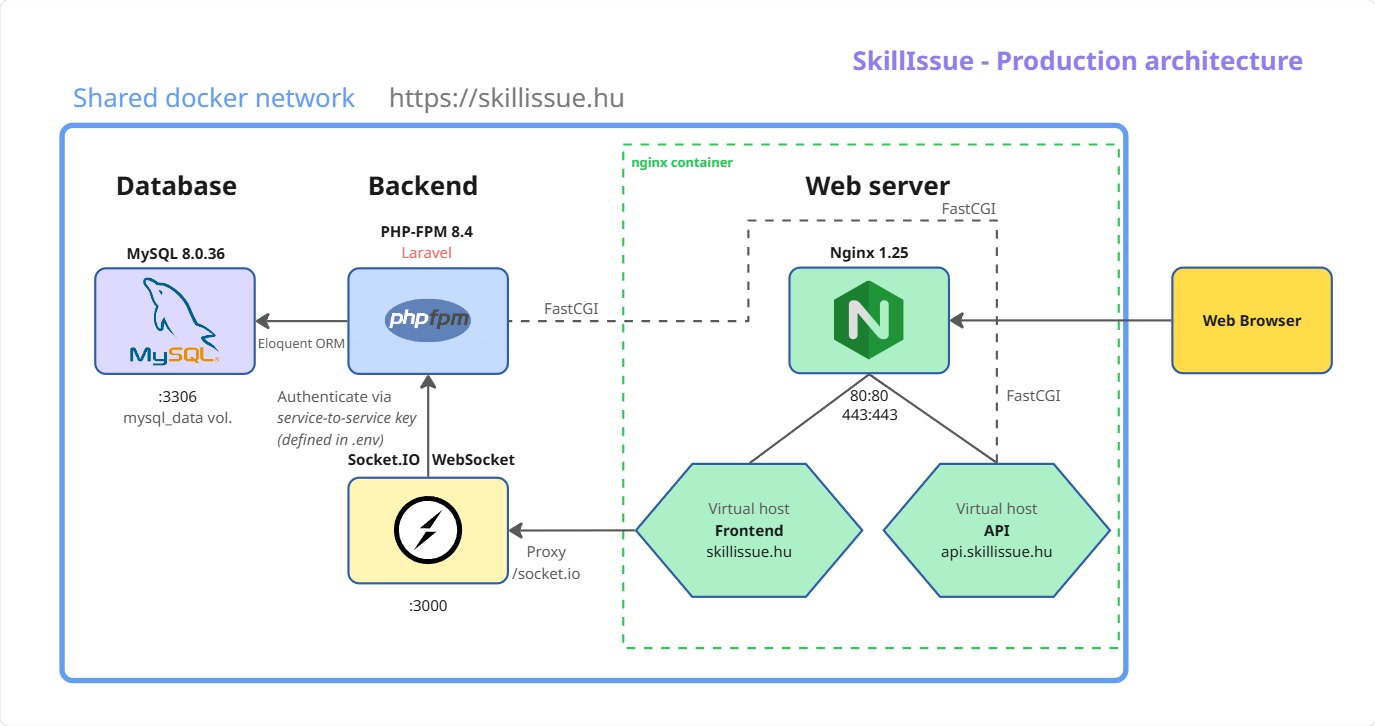
\includegraphics[width=\textwidth]{images/prod_diagram.png}
    \caption{A SkillIssue éles környezetének architektúrája}
    \label{fig:architektura}
\end{figure}
\chapter{Technológiák}

\section{Backend - Laravel}
A Backend oldalon a megvalósítás a PHP nyelvre épül, azon belül is a \textbf{Laravel} keretrendszer köré.

\begin{description}
    \item[Autentikáció]A Sanctum csomag használatával valósul meg az autentikációs réteg. Előnye, hogy egyszerűen használható, lightweight megoldás. Mivel a SkillIssue alkalmazás csakis webes megvalósítással rendelkezik, Cookie alapú session autentikáció mellett döntöttünk. Az API a REST elveit követi, kivéve az autentikációs réteget, ahol a bejelentkezett felhasználó session-je
    tárolódik.
    \item[EloquentORM]ORM használata megkönnyíti a fejlesztői munkafolyamatot, azáltal, hogy migration-ökben tárolódnak az adatbázis táblák sémái, és osztályok példányain érhetőek el az entitások. Kiküszöböli az SQL injection veszélyeit, mivel nem nyers SQL utasításokra épül a rendszer.
    \item[PHP-FPM/FastCGI]Gyors, skálázható kiszolgálási forma az API számára
    \item[MySQL]Azért esik a MySQL adatbázisra a választás, mert gyors lekérdezéseket és könnyű integrációt biztosít a Laravel-lel. Más lehetséges megoldások, például a SQLite, azért nem kerül alkalmazásra, mivel kevésbé skálázható adatbázis megoldásokat biztosít.
    \item[JWT tokenek]Az alkalmazás a JWT tokeneket nem autentikációhoz használja, hanem 3 különböző tokent képes kiállítani a megfelelő lekérdezések alkalmával: Kérdés token, egyjátékos meccs token, és rangsorolt (1 vs. 1) meccs token. Ezekre a megoldásokra azért van szükség, hogy kódolt formában tudjon adatot továbbítani a kliens számára, és ne plaintext formában küldjön fontos adatokat. Továbbá, a JWT tokenek működési elvéből adódóan könnyen kezelhető a tokenek lejárati ideje, így például lehetőség van a megoldás beküldésének elutasítására, amennyiben a kérdés token lejár.
    
\end{description}

\newpage

\section{WebSocket - Node.js}
A WebSocket megvalósítása a Socket.IO csomaggal történik. Az említett csomagnak az előnye, hogy könnyen kiépíthető a WebSocket kapcsolat, emellett lehetőséget biztosít HTTP Polling fallback-re, amennyiben a kliens nem képes WebSocket kapcsolatot kezdeményezni.\\
A WebSocket megvalósítása nem tartalmaz üzleti logikát, és adatbázis módosítást nem végez. Ezek helyett az API-val kommunikál.

\begin{description}
    \item[WebSocket $\rightarrow$ API kapcsolat]A WebSocket és a Laravel API közös környezeti változókból dolgozik. Ez teszi lehetővé, hogy egy közös token-t tudnak olvasni, amelyet service-to-service tokenként nevezünk. Ez egy konstans token, amely nem tárol semmilyen adatot, csupán validációra szolgál, mivel az összes \texttt{/api/internal/}-al kezdődő útvonalat csakis a WebSocket veheti igénybe, felhasználó közvetlenül nem.
    \item[Felhasználó autentikáció]A WebSocket külön, belső API útvonalon autentikálja a felhasználót. Ennél a folyamatnál kihasználja azt, hogy a sütik minden lekérésnél továbbmennek a lekérés helyére. Ezáltal a cookie-kat manuálisan elküldve egy belső útvonalnak, könnyedén kinyerhetőek a felhasználó adatai.
    \item[Állapotkezelés]Az ideiglenes állapotkezelésre a legegyszerűbb módot alkalmazza a rendszer, így Hash Map formájában tárolja a különböző adatokat, amelyek a következők: Meccskeresési queue, megerősítésre váró meccsek\footnotemark és folyamatban lévő meccsek. Ennek a tárolási módszernek a legnagyobb hátránya, hogy ha a WebSocket szolgáltatás váratlanul újraindul, a folyamatban lévő meccsek elvesznek, ezáltal nem befejezhetőek. \textit{Ilyenkor Elo változás nem történik.}
\end{description}
\footnotetext{A két játékosnak, akiket a Matchmaking rendszer összesorol, meg kell erősíteni a játszmát - Ne kezdődjön el úgy meccs, hogy egyik felhasználó nincs a számítógép előtt (AFK).}


\section{Frontend - Vue.js}
A Frontend szolgáltatáshoz a Vite build tool-t alkalmazza a rendszer, ami fejlesztői környezetben lehetővé teszi a projekt gyors elindítását, fejlesztői webszervert futtat, és hot reload funkciót is biztosít.\\
Mivel a SkillIssue egy közepes méretű projekt, a Vue.js egy gyors, egyszerű és átlátható fejlesztési folyamatot biztosít. Más keretrendszerek, például az Angular azért nem kerül alkalmazásra, mert a projekt méretéhez képest indokolatlanul komplex megoldás lenne.

\begin{description}
    \item[Útvonalválasztás]A routing problémáját a Vue Router oldja meg, ami a standard megoldás egy Vue alkalmazás esetében. Lehetővé teszi, hogy átirányítson, URL paramétereket fogadjon, és metaadatot kapcsoljon bizonyos oldalakhoz (például vendég elérheti-e).
    \item[Állapotkezelés]A prop drilling elkerülése érdekében a Pinia csomagot alkalmazza a rendszer, ami egy Vue.js-re szabott állapotkezelő megoldás. A Pinia került alkalmazásra a projekt megvalósítása során, mivel ez az egyik legkönnyebben használható store csomag a Vue ökoszisztémában. Emellett a hivatalos Vue dokumentáció is a Pinia Store-t javasolja, illetve jól integrálható a Vue Dev Tools kiegészítővel is.
    \item[WebSocket kliens oldalon]A WebSocket kapcsolatot a Frontend bejelentkezéskor kezdeményezi, vagy már bejelentkezett felhasználó esetén akkor, amikor validálásra kerül a felhasználó bejelentkezett állapota. Ez teszi lehetővé, hogy az alkalmazás érzékelje a már megkezdett meccseket, és automatikusan visszacsatlakoztassa a felhasználót a folyamatban lévő többjátékos meccsbe. A meccskeresés és játékmenet elkülönítve, store-ban kerül tárolásra. Itt futnak azok a listener-ök is, amelyek figyelik a WebSocket felől érkező eseményeket.
    \item[HTTP Kérések]Az API-hoz intézett kérések kezeléséhez az Axios csomagot alkalmazza a projekt. Ennek előnye, hogy megkönnyíti a HTTP kérések folyamatát a JavaScript-be beépített fetch API-hoz képest. Saját Axios példányt alkalmaz a projekt, ezáltal letisztultabb, átláthatóbb kódot biztosít, hiszen bizonyos szükséges fejlécek automatikusan kitöltésre kerülnek.  
    \item[Design]A projekt megvalósítása során felhasználásra került a Tailwind CSS keretrendszer, amely egyszerűbbé teszi az oldalon megjelenő elemek stílusának személyre szabását. A Tailwind kellő szabadságot biztosít a fejlesztőnek, hogy egyedi Design-t alkothasson, szemben olyan framework-ökkel, mint például a Bootstrap, ami sokkal szigorúbb keretek közé szorítja a design-t. A projekt egy letisztult, konzisztens, glassmorph elemekkel díszített arculatot valósít meg. A színpaletta élénk színeket tartalmaz, amely tovább fokozza az oldal játékos hangulatát. A Tailwind mellett a FontAwesome ikonkönyvtár ingyenes verziója lett alkalmazva, a nagy választék miatt. A FontAwesome CDN linken keresztül kerül beágyazásra.
\end{description}

\newpage

\section{Konténerizáció - Docker}
\label{sec:dockeconfig}
\begin{description}
    \item[Döntés indoklása]Két fős projektként a Docker megkönnyíti a fejlesztési  folyamatot, mivel azonos környezeten tudnak dolgozni a csapattagok. Ezzel elkerülve azt a gyakori problémát, hogy az egyik számítógépen működik, a másikon pedig nem, például verziókülönbség miatt.
    \item[Megvalósítás]A projekt Docker Compose-t használ, ezáltal könnyedén futtatható több szolgáltatás egyszerre, összehangolt módon. A két környezet (production, development) külön compose fájlokban van definiálva. 
    \item[Fejlesztői környezet elvárásai]Könnyen elindítható, fejlesztő-barát megoldás megvalósítása. A hot-reload támogatása és a host számítógép és a konténer közötti jogosultságok szinkronizálása, különösen az \texttt{artisan} parancssori eszköz esetében, hiszen az képes fájlokat létrehozni a host számítógépen. Ezek miatt szükséges a volume-ok kialakítása, amivel a hot-reload és a MySQL hosszú távú adattárolása megvalósulhat. A jogosultságok érdekében a host felhasználó Group ID és User ID értékeit használja a konténer is.
    \item[Éles (production) környezet elvárásai]Egyszerű szállítás és deployment. Megoldásként a Makefile parancsai szolgálnak, amelyek lehetővé teszik, hogy egyszerűen egy paranccsal kiadható legyen egy új verzió. A másik fontos szempont a biztonság, ezért ahol csak lehetséges, non-root felhasználó van konfigurálva a konténerben. A gyors kiszolgálás és proxy-zás érdekében nginx webszerver került alkalmazásra. Az nginx a Cloudflare origin SSL-t alkalmazza, a HTTPS kapcsolat kiépítésének érdekében. A konfiguráció továbbá lehetővé teszi, hogy ameddig az alkalmazás tesztelési fázisában van, jelszóval védett legyen a virtuális hoszt. További információ: \ref{fig:architektura}. ábra
    
\end{description}
\section{Adatbázis-terv}
\label{sec:adatbazis}

\subsection{ER Diagram}
Az adatbázis szerkezeti felépítését és az entitások közötti kapcsolatokat az alábbi ER (Entity-Relationship) diagram szemlélteti. A diagram a DrawDB eszközzel készült. Online elérhető  \href{https://www.drawdb.app/editor?shareId=650aa51fedc729b51f89df3084050733}{ide kattintva}.

\begin{figure}[htbp]
    \centering
    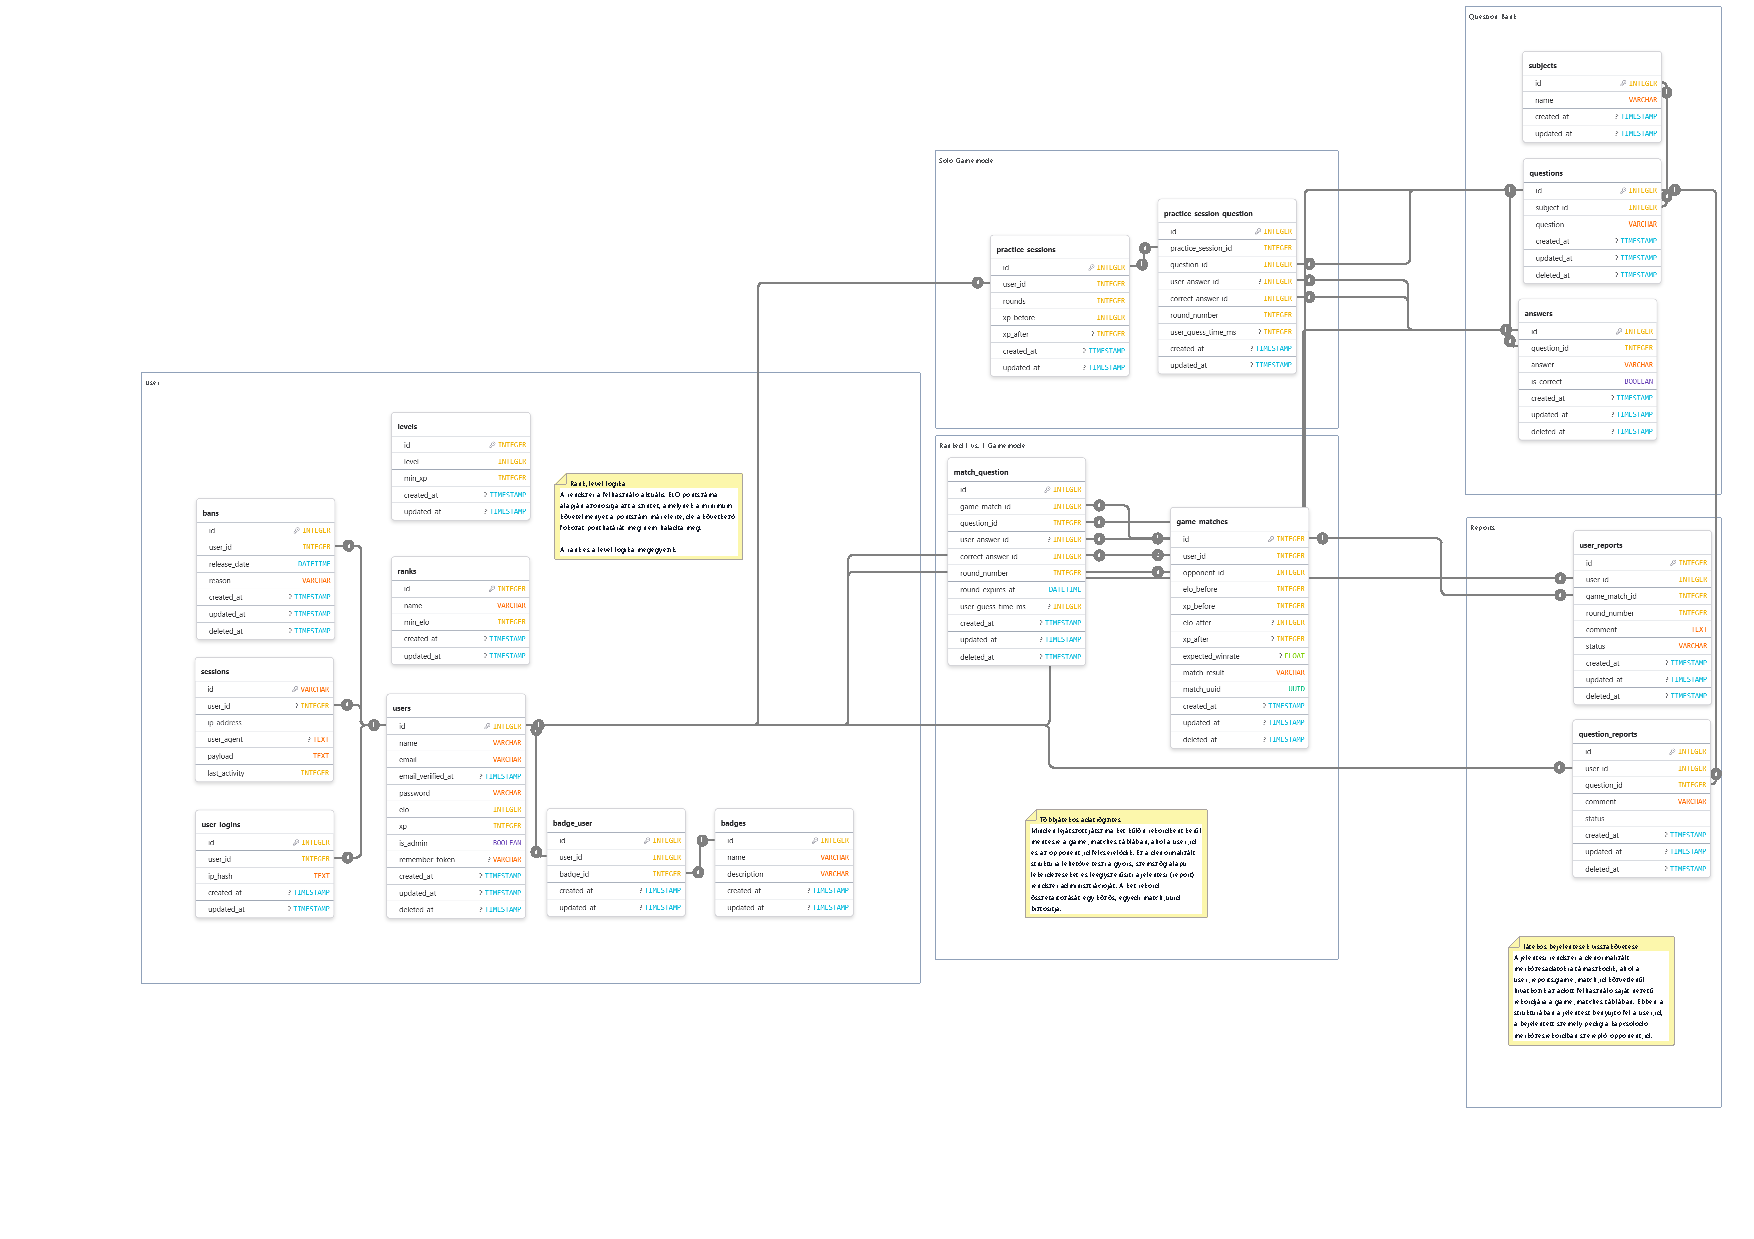
\includegraphics[width=\textwidth]{images/er-diagram.pdf} 
    \caption{A SkillIssue alkalmazás ER diagramja}
    \label{fig:er_diagram}
\end{figure}

\subsection{Entitások leírása}
A rendszer főbb entitásai és azok szerepkörei:

\begin{itemize}
    \item \textbf{users:} A felhasználók alapvető adatait, kompetitív rangját (ELO), tapasztalati pontjait (XP) és adminisztrátori jogosultságait tárolja.
    \item \textbf{questions \& answers:} A kvízjáték magját alkotó kérdések és a hozzájuk tartozó helyes/helytelen válaszlehetőségek tárolóhelye, tantárgyak (subjects) szerint csoportosítva.
    \item \textbf{game\_matches:} A felhasználók közötti párbajok adatait rögzíti. A gyors lekérdezhetőség és az adatbázis kapcsolatok egyszerűsítésének érdekében redundáns (denormalizált) módon tárolja a meccseket, minden résztvevő szemszögéből egy-egy rekorddal.
    \item \textbf{match\_question:} A mérkőzések során feltett konkrét kérdéseket, a felhasználó válaszait és a válaszidőket rögzíti körökre bontva.
    \item \textbf{practice\_sessions:} A gyakorló mód adatait tárolja, ahol a felhasználó tét nélkül (ELO változás nélkül) szerezhet tapasztalatot.
    \item \textbf{reports:} Felhasználó és kérdés jelentések kezelésére szolgáló entitások a platform moderációjához.
    \item \textbf{bans \& logins:} Biztonsági entitások, amelyek a kitiltások és a bejelentkezési előzmények (IP hash) nyomon követésére szolgálnak.
\end{itemize}

\subsection{Kapcsolatok és megszorítások}
Az adatbázis integritását az alábbi főbb kapcsolatok és megszorítások biztosítják:

\begin{enumerate}
    \item \textbf{Egy-a-többhöz (1:N) kapcsolatok:}
    \begin{itemize}
        \item Egy \texttt{subject} több \texttt{question}-höz kapcsolódik.
        \item Egy \texttt{question}-höz több \texttt{answer} tartozik.
        \item Egy \texttt{user} több mérkőzéssel (\texttt{game\_matches}), gyakorlással (\texttt{practice\_sessions}) és jelentéssel rendelkezhet.
    \end{itemize}
    
    \item \textbf{Több-a-többhöz (N:M) kapcsolatok:}
    \begin{itemize}
        \item A felhasználók és badge-ek kapcsolata a \texttt{badge\_user} kapcsolótáblán keresztül valósul meg.
    \end{itemize}

    \item \textbf{Egyediségi megszorítások (Unique):}
    Az e-mail címek, a rangok minimum pontszámai (\texttt{min\_elo}) és a szintek (\texttt{min\_xp}) egyedisége biztosítja, hogy a rangsorolási és azonosítási rendszer egyértelmű maradjon.
    
    \item \textbf{Denormalizációs stratégia:}
    A \texttt{game\_matches} tábla szándékosan duplikált rekordokat tárol (minden meccset kétszer, felcserélt \texttt{user\_id} és \texttt{opponent\_id} mezőkkel), amit egy közös \texttt{match\_uuid} fog össze. Ez egyszerűsíti a lekérdezési folyamatot több adatbázis kapcsolaton keresztül.
\end{enumerate}
\chapter{Backend - API}

\section{Autentikáció}
A SkillIssue a felhasználó autentikációjához a Sanctum csomagot használja, azon belül is cookie alapú session autentikációt. Ennek az az előnye, hogy a kérésekkel automatikusan elküldődik a süti, így könnyen azonosítható a felhasználó egyéb fejlécek megadása nélkül. A projekt megvalósítása webes felületen történik, ezért nincs szükség a JWT és egyéb autentikációra szolgáló tokenek sokoldalúságára, viszont a jövőbeli igények figyelembevételével később jó fejlesztési lehetőség lehet.

\section{Felhasználókezelés}
A felhasználókról a következő információk kerülnek tárolásra:
\begin{itemize}
    \item Név
    \item Email
    \item Jelszó (Bcrypt hash)
    \item ELO
    \item XP
    \item Adminisztrátori jogosultsággal rendelkezik-e?
    \item Bejelentkezésekhez tartozó IP címek (hash-elt formában, csupán összehasonlításra)\footnotemark
\end{itemize}

A felhasználókat továbbá ki lehet tiltani a rendszerből, ez valójában egy új adatbázis-rekord létrehozását jelenti a \texttt{bans} táblában. Amennyiben a felhasználónak aktív kitiltása van, a rendszer nem engedi játszani, és tájékoztatja a kitiltás indokáról és annak lejáratáról.

\footnotetext{A rendszer a $V\curversion$ verzióban nem használja fel a tárolt IP címeket semmilyen módon. Jövőbeli fejlesztési lehetőségek megalapozására kerülnek tárolásra.}


\section{Kérdéskezelés}
A kérdéseket lekérni normál felhasználónak nincs jogosultsága, csak az adminisztrátoroknak. Az adminisztrátor jogosultsággal rendelkező felhasználók kérdéseket módosíthatnak, törölhetnek, vagy adhatnak hozzá - már létező, vagy új tantárgy megadásával. 
\\
Normál felhasználó csak akkor kérhet le kérdést, amennyiben aktív játékmenetben van (JWT tokennel azonosítva) és a \texttt{/api/questions/get-one} útvonalat használja. Ez egy véletlenszerűen választott kérdést ad vissza (amelyet a felhasználó még nem látott a meccs során) a válaszokkal együtt.

\newpage
\section{Meccs és kör logika}
\subsection{Egyjátékos mód}

Játszma folyamata lépésről lépésre: 
\begin{enumerate}
    \item \textbf{Indítás:} A játékos elindítja a játszmát. Ilyenkor az API felé kérést indít (POST \texttt{/practice-sessions}), ami elkészíti a játszmát az adatbázisban, illetve létrehozza a JWT token-t (\textit{GameToken}), ami a játszma azonosítására szolgál az API és a Frontend kommunikációjában. A token eltárolja a felhasználó azonosítóját és az elkészített játszma azonosítóját. Amennyiben a felhasználó aktív kitiltás alatt áll, a játszma nem lesz létrehozva, és az API 403-as hibával tér vissza.
    \item \textbf{Átirányítás:} A játékos átkerül egy új oldalra, amelyen az URL paraméterben a játszma JWT tokenje található meg. Ez biztosítja, hogy amennyiben elhagyja a játékot, vissza tud lépni, és nem veszti el a teljes előrehaladását.
    \item \textbf{Kérdés lekérése:} A kör elején a Frontend POST kérést küld a \texttt{/api/questions/get-one} útvonalra, amely válaszol a véletlenszerűen kiválasztott kérdéssel, illetve az azokra eltárolt lehetséges válaszokat is visszaadja, összekevert sorrendben. A kérés csak akkor végződik sikeresen, ha a játszma elkészítésekor létrehozott JWT token el lett küldve, és megfelelő (felhasználó azonosító egyezik a kérést elküldő felhasználóéval). Új JWT token kerül kiállításra (\textit{QuestionToken}), amely tartalmazza a kérdés és a felhasználó azonosítóját. 
    \\
    Amennyiben az adatbázisban nincs elegendő kérdés \textit{(körök száma > kérdések száma)}, a játszma csak addig folytatódik, ameddig el nem fogynak a felhasználó által (az adott játszmában) még nem látott kérdések; ezek után hibát ad.
    \item \textbf{Válaszadás:} Amennyiben a játékos be kívánja küldeni a válaszát, ki kell választani az általa helyesnek vélt választ, majd az alsó \textit{"Beküldés"} gombra kattintva elküldeni a szervernek. Ilyenkor POST kérés fog végbemenni a \texttt{/api/answers/verify/\{válasz azonosító\}} végpontra, mely kötelezően elvárja a QuestionToken-t és a GameToken-t. Amennyiben a válasz azonosító helyén a \texttt{null} literál szerepel, az eltárolt válasz is \texttt{NULL} értékű lesz, ez jelzi, hogy a felhasználó nem adott választ időben. A kérésre válaszként megérkezik, hogy a válasz helyes volt-e, illetve hogy mi lett volna a helyes válasz. Amennyiben a játékos az utolsó kérdésre válaszolt, visszaadja a megszerzett XP pontokat is ($n_{\text{helyes válaszok}} \cdot 10$). Amennyiben a felhasználó nem küldi be magától az idő leteltével a válaszát, a rendszer automatikusan beküldi a kiválasztottat - ha van olyan - egyébként üres választ küld be (\texttt{null}).
\end{enumerate}

\subsection{Többjátékos (Rangsorolt 1 vs. 1) mód}
A többjátékos módhoz a lekéréseket a WebSocket szolgáltatás végzi, a belső \texttt{/api/internal} előtaggal ellátott végpontokra. 
\\Ezek a végpontok a következők:
\begin{itemize}
    \item \texttt{/game-matches}: A törzsben 2 paramétert kaphat: \texttt{user\_a\_id} és \texttt{user\_b\_id}. Amennyiben a felhasználók közül valamelyik jelenleg aktív kitiltás alatt van, a játszma nem lesz létrehozva, és 403-as hibakóddal tér vissza az API. Adatbázis tranzakcióban kezeli a meccs létrehozását a rendszer, ugyanis egy játszma két adatbázis rekordnak felel meg (Részletek: \ref{sec:adatbazis}. szakasz). Ez kiküszöböli annak lehetőségét, hogy az egyik meccs létrehozásra kerüljön, a másik viszont sikertelen legyen. A JWT token payloadjában a következő adatok szerepelnek: Egyedi meccsazonosító, A felhasználó azonosítója és B felhasználó azonosítója. A rendszer továbbá kiszámolja a várt nyerési arányt a játékosoknak, a \ref{sec:pontozas} szakasz alapján, majd visszaküldi a két felhasználó nevét, hogy a játékosok ismerhessék az ellenfelüket.
    \item \texttt{/questions/get-one}: Arra szolgál, hogy a WebSocket lekérhesse a következő kérdést, amit feltesz a játékosoknak. A rendszer kezeli, hogy olyan kérdéseket kapjanak a játékosok, amit még nem láttak az adott játszmában, valamint azt, hogy a válaszok sorrendje összekevert legyen. A rendszer azt is kezeli, hogyha tévesen bejönne még 1 kérés egy olyan meccsre, ami már véget ért (következő kör > maximum körök). Kiállít egy \texttt{QuestionToken}-t, a két felhasználó azonosítójával, valamint a kérdés azonosítójával.  Tranzakcióban bejegyzi az adatbázisba a kérdéseket, a lejárati idejükkel együtt.
    \item \texttt{/answers/verify/\{válasz azonosító\}}: Arra szolgál, hogy visszaadja a helyes választ az adott kérdésre, bejegyezze a felhasználó válaszát és kezelje a játszma lezárását (ha az utolsó körben érkezik a kérés). A beküldő felhasználó azonosítója a kérés törzsében érkezik. A rendszer kezeli, ha olyan felhasználó küld be választ, aki nem vesz részt azon a játszmán, illetve azt is, ha nem küld be választ a felhasználó (\texttt{NULL}). A rendszer továbbá azzal is foglalkozik, ha a válasz nem az adott körben következő kérdéshez tartozik, továbbá figyelembe veszi a kérdés lejáratát is. Az adatbázisban a felhasználó válaszadási idejét is tárolja a rendszer, amit a kérdés elkészítési időbélyegből és a szerveridőből számol. A rendszer nem korrigál a felhasználó hálózati késleltetése alapján, sem az adatbázis lekérésének sebességével - nagyságrendileg a valóságnak megfelelő értéket tárol. Amennyiben az utolsó válasz kerül beküldésre, a rendszer kiszámolja az eltárolt várható nyerési esély alapján az ELO nyereséget/veszteséget, majd visszaküldi azt, a helyes válasszal együtt.
\end{itemize}
\textbf{Megjegyzés:} A többjátékos módhoz tartozó \texttt{/api/internal} előtagú végpontok nem ugyanazokat a controllereket használják, mint az egyjátékos módban, annak ellenére, hogy nevük ugyanaz. Az elnevezés oka a két játékmenet logikájának hasonlóságán alapszik.


\section{Bejelentő rendszer}
Két fajta bejelentést különböztet meg a rendszer: játékos bejelentés és kérdés bejelentés.

\subsection{Játékos bejelentés}
Bármelyik játékos bejelentheti az ellenfelét az 1 vs. 1 rangsorolt meccsek folyamán. Olyan személyek bejelentésére nincs lehetőség, akikkel nem játszott együtt a játékos. Az adatbázis tárolja a bejelentéseknél többek között azt, hogy melyik körben lett jelentve az ellenfél (a könnyebb kivizsgálás érdekében), de ezt a felhasználó felülírhatja, hogy melyik volt számára a leggyanúsabb kör. Emellett szöveges leírást is adhat az eseményről. 

\subsection{Kérdés bejelentés}
Amennyiben a felhasználó egy adott kérdést és/vagy az azokra megadott válaszokat helytelennek találja, esetleg hibás "helyes válasz" van megjelölve, bejelentést tehet. Szöveges megjegyzés formájában leírhatja mi volt a probléma az adott kérdéssel. 

\subsection{Kérdések elbírálása}
Az alábbi állítások mind a kérdés -és a játékos bejelentésekre igazak.
\begin{itemize}
    \item Normál felhasználó csak POST kéréseket küldhet a végpontokra; más, illetve saját bejelentéseit nem tekintheti meg.
    \item Az adminisztrátor jogosultsággal rendelkező felhasználók egy külön felületen tekinthetik meg a beérkezett jelentéseket. Azok státuszát (nyitva, vizsgálat alatt, lezárva) módosíthatják, reportokat törölhetnek. Játékos bejelentés esetében látják a felhasználó statisztikáját is, kérdés bejelentésnél pedig a kérdést és a hozzá tartozó válaszokat. Az adminisztrátorok saját megjegyzésüket is odaírhatják a felhasználóé mellé, így jelezve a többi adminisztrátornak észrevételüket.
\end{itemize}

\section{Service-to-service kommunikáció}
A több szolgáltatáson keresztül való kommunikációk validálására az API az \texttt{EnsureServiceTokenIsValid} nevű middleware-t használja. Ennek feladata mindössze annyi, hogy összehasonlítsa a \texttt{.env} fájlban meghatározott kulccsal a fejlécben megadott Bearer token-t.


\chapter{WebSocket szerver}

\section{Miért külön szolgáltatás}
A SkillIssue alkalmazás a WebSocket szervert külön szolgáltatásként definiálja. A cél elérésére a Socket.IO csomagot használja. Ennek okai az alábbiak:
\begin{itemize}
    \item Az API-tól függetlenül skálázható megoldás.
    \item Amennyiben az API újraindul, a WebSocket szolgáltatás továbbra is elérhető marad. Emiatt a folyamatban lévő meccsek nem szakadnak meg, és a legtöbb esetben tovább folytathatók.
    \item Feladatkörök szétválasztása
\end{itemize}

\section{Kapcsolat az API-val}
Az API kommunikáció során az axios példányban meghatározott fejlécek kerülnek elküldésre, amelyekből kiemelten fontos az \texttt{Authorization} header. Ez tartalmazza a service-to-service token-t.
\\
A felhasználó azonosításához egy middleware áll rendelkezésre a WebSocket-en belül, amely a kapott cookie-k alapján az API-val való kommunikáció után eltárolja a felhasználó adatait.
Ezek után a kommunikáció a REST standard szerint történik.

\section{Valós idejű meccs folyamat}
A folyamat a következők szerint zajlik:
\begin{enumerate}
    \item A felhasználó csatlakozik a WebSocket-hez. Amennyiben van aktív játszma hozzárendelve, a WebSocket elküldi ezt a kliensnek, ami automatikusan visszacsatlakoztatja.
    \item Amennyiben nincs aktív meccs folyamatban, a felhasználó csatlakozhat a Matchmaking Queue-hoz. Ekkor bekerül egy hash map struktúrában tárolt sorba, amit a WebSocket 2 másodpercenként kiértékel \textit{(\ref{sec:matchmaking} fejezet alapján)}.
    \item Amennyiben sikeresen párosításra kerül 2 játékos, létrejön egy \texttt{Pending match}, amelyet mindkét játékosnak el kell fogadnia. Amennyiben elfogadja, csak akkor kerül át az \texttt{ongoingMatches} hash map-be, és kerül létrehozásra a játszma az adatbázisban.
    \item Lekérésre kerül egy kérdés, majd ez megjelenítésre kerül a játékosok előtt (mindkét játékos ugyan azt a kérdést kapja).
    \item Amennyiben egy játékos elküldi a válaszát, kiértékelésre kerül, de még nem látja meg, hogy helyesen válaszolt-e, mindaddig amíg a másik játékos el nem küldi válaszát. Ez idő alatt a WebSocket emit-el egy eseményt, ami által a frontend meg tudja jeleníteni a feliratot: \textit{"Várakozás [Játékos neve] válaszára"}.  
    \item Amennyiben mindkét felhasználó válaszol, a WebSocket emit-eli a helyes választ, ami megjelenítésre kerül a felhasználók számára. Ezután rövid várakozással a folyamat újraindul a következő kérdéssel. Amennyiben nincs már több kérdés, tehát az utolsó kört játszották, az utolsó válasz beküldése után a játszma kiértékelésre kerül, és a felhasználónak ezt a WebSocket elküldi. A kiértékelést az API végzi, nem a WebSocket. Ilyenkor a felhasználót átirányítja az összegző felületre, ahol láthatja a meccset, és akár meg is tudja osztani másokkal az eredményt.
    \item Kikerül a játszma az \texttt{OngoingMatches} hash map-ből.
\end{enumerate}

\begin{description}
    \item[Matchmaking] Amennyiben a játékos már meccskeresési queue-ban van, nem léphet be újra. Ugyanez a helyzet, ha már van aktív játszma a felhasználónak.
    \item[WebSocket kapcsolat] Amennyiben a felhasználó több lapról nyitotta meg a böngészőben a SkillIssue alkalmazást, csak az egyikben lesz aktív WebSocket kapcsolata, így a másikról a real-time játékmenet nem fog működni.
\end{description}
\chapter{Frontend}
A projekt Frontend megoldása Vue.js-en, annak is a modern Composition API-án alapul. Azért a Vue.js-re esett a választás más keretrendszerek helyett, mert a Vue olyan megoldásokat biztosít, amelyek egy kis-közepes projekt számára előnyösebbek. Könnyebb tiszta, jól átlátható és egyszerűen fenntartható kódot írni, mint egy komplexebb keretrendszerben (pl. Angular, React). Emellett a támogatása is kiemelkedő, olyan csomagokkal, mint például a Pinia és a Vue Router.

\section{Oldalak és navigáció}
A navigációhoz a Vue Router csomagot használja az alkalmazás. Több előnye is van ennek a megoldásnak:
\begin{enumerate}
    \item Az oldalak nem töltődnek újra, csak a komponensek cserélődnek ki
    \item Lehetőség van Eager- és Lazy loading alkalmazására is
    \item Könnyen megoldható a jogosultságok ellenőrzése
    \item Jól bevált ipari standard
\end{enumerate}
A Vue Router-ben a \texttt{WebHistory} előzménymódot használja az alkalmazás, mivel ez ideális egy SPA számára. 

\section{Komponensstruktúra}
A Frontend kódbázis mappastruktúrájának kialakításakor elsődleges szempont az átláthatóság és a könnyű kezelhetőség. Ennek érdekében a komponensek külön \texttt{components} könyvtárban helyezkednek el. Ezen könyvtáron belül altípusok mappái találhatóak, pl.: Auth, Dashboard, Game, Generic. A komponensek elkészítése során fő szempont a modularitás, így kiemelt szerepet kapnak a prop-ok a komponensek kiépítésében.

\section{Állapotkezelés}
A prop-drilling megakadályozására Pinia store-t használ a rendszer, amelyek a kódbázis \texttt{stores} könyvtárában helyezkednek el. A kialakításuk során fontos szempont, hogy a Single Responsibility Principle-nek megfeleljenek, azaz csak egy jól körülhatárolt feladatot végezzenek. A következő állapotkezelésre alkalmas store-ok találhatóak meg a projektben:
\begin{description}
    \item[UserStore] A felhasználó bejelentkeztetése, azonosítása, kijelentkeztetése, és adatinak tárolása.
    \item[MatchmakingStore] WebSocket kommunikáció létesítése, események kezelése, meccskeresés elindítása, befejezése, átirányítás a játék oldalra találat esetén.
    \item[GameStore] Minden játék közbeni esemény lekezelése, válasz beküldése, új kérdés fogadása, felhasználó visszacsatlakoztatása folyamatban lévő játszma esetén.
\end{description}

\section{WebSocket integráció kliens oldalon}
\subsection{Konfiguráció}
Frontend oldalon az alkalmazás a Socket.IO kliensének NPM csomagját használja. Olyan módon van konfigurálva, hogy amennyiben a felhasználó böngészője támogatja a WebSocket kapcsolatokat, elsődlegesen azt használja, de fallback-ként HTTP polling-ra is képes.

\subsection{WebSocket kapcsolat}
A WebSocket kapcsolat akkor jön létre, amikor a felhasználó megnyitja az oldalt. Amennyiben több mint egy lapról van megnyitva a skillissue.hu oldal egy felhasználó alatt, a megfelelő működés csak az elsőként megnyitott lapon garantált. Kivétel ez alól az összes bejelentő oldal, amelynél külön kikapcsolásra kerül a WebSocket kapcsolat annak érdekében, hogy a bejelentő oldal a folyamatban lévő játékmenetet ne zavarja. 

\subsection{Eseménykezelés}
A WebSocket kliensnek érkező eseményeket az adott eseményhez kapcsolódó Pinia store figyeli. Hiba esetén (pl. WebSocket szolgáltatás megáll) értesíti a felhasználót a rendszer, és leállítja a folyamatban lévő meccskeresést (amennyiben van ilyen).
\chapter{Játékmechanika}
A rendszer alapvetően két játékformát valósít meg: Egyjátékos gyakorló mód és Rangsorolt többjátékos (1 vs. 1) mód. 

\section{Egyjátékos mód}
Tét nélküli gyakorló játékmód. A felhasználó feleletválasztós kérdéseket kap, ahol csak egy jó válasz lehetséges. Adott időn belül válaszolnia kell a kérdésre. Amennyiben nem válaszol, üres válasz lesz eltárolva, és nem kap érte pontot. Válaszadás esetén (legyen az üres válasz, vagy a felhasználó által kiválasztott) a következő kérdés automatikusan lekérésre kerül, miután a rendszer megmutatta a helyes választ a felhasználónak. Ez a folyamat a konfigurációtól függően $n$ körig folytatódik. Az utolsó kör végén a válasz beküldésével a rendszer összesíti a helyes válaszokat és ennek megfelelően XP-vel jutalmazza a játékost, ahol minden helyes válasz után 10 XP jár. Negatív végeredmény nincsen, a rendszer XP-t vagy bármi más pontot nem von le a játékostól.
\section{Rangsorolt 1 vs. 1 mód}
Rangsorolt játszma, azaz XP mellett ELO pontokat is szerezhet a játékos; viszont itt már negatív eredmény is kerülhet számításra az ELO esetében.
\\
A játékos belép a meccskeresési folyamatba (bővebben: \ref{sec:matchmaking}. szakasz). Amikor a rendszer megfelelő ellenfelet talál a felhasználónak, el kell azt fogadnia, ezzel megerősíti, hogy a számítógép előtt tartózkodik, és készen áll a meccsre. Amennyiben nem erősíti meg valamelyik játékos, a meccskeresés számukra leáll, és jelzi a rendszer, hogy legalább az egyik játékos nem fogadta el a játszmát. Amennyiben mindkét játékos elfogadja, továbbjutnak a játék oldalra.
\\
Az egyjátékos módhoz hasonlóan, feleletválasztós formában kapnak kérdéseket. Mindkét játékos ugyan azt a kérdést kapja, ugyan azokkal a válaszokkal. Szintén, egy helyes válasz lehetséges az adott kérdésnél. A játékosoknak megadott idő áll rendelkezésre, hogy beküldjék a válaszukat. Amennyiben az idő letelik, vagy mindkét felhasználó beküldi a válaszát az idő letelte előtt, a rendszer sárga színnel jelzi a felhasználó válaszát, lilával az ellenfél válaszát, és zölddel a helyes választ. Amennyiben a helyes válasz, a felhasználó válasza, és az ellenfél válasza közül legalább kettő ugyan az a válasz, a háttérszínük megoszlik, kettő vagy három részre. Például, ha a legelső volt a helyes válasz, és a felhasználó, valamint az ellenfél válasza is, akkor az első válasz háttérszínének első harmada sárga, második harmada lila, és utolsó harmada zöld háttérszínű lesz, így jelezve a felhasználónak, hogy mindenki a helyes választ küldte be.
\\
Amennyiben az idő letelik, és van megjelölt, de még nem beküldött válasza valamelyik felhasználónak, a rendszer automatikusan beküldi azt. Ha nincs, üres válasz kerül beküldésre. Ilyenkor a következő kör automatikusan indul.
\\
Az utolsó kör végén, amikor mindkét felhasználó beküldte a válaszát, vagy letelt az idő, a rendszer összegzi a játszmát, és kiszámítja a hozzáadott és levont pontokat, valamint a nyertest (Bővebben: \ref{sec:pontozas}. szakasz).

\newpage
\section{Matchmaking folyamat}
\label{sec:matchmaking}
A meccskeresés úgynevezett képességalapú párosítást használ (SBMM\footnotemark).
\footnotetext{A Skill Based Matchmaking (képességalapú párosítás) olyan párosító rendszer, amit gyakran játékok használnak arra, hogy minden félnek élvezetes és kompetitív élményt nyújtsanak - egyik játékos se érezze, hogy hatalmas hátrányban van ellenfelével szemben.}
\\
Működése: Konstans változók tárolják azokat az értékeket, amik befolyásolják, milyen a játszma, ami a leginkább unfair, de még az elfogadható tartományba tartozik. A következők kerülnek definiálásra:
\begin{description}
    \item[Base elo range] Az alapbeállítás, ekkora ELO különbségben keresi az ellenfelet a játékosnak a rendszer. 
    \item[Maximum elo range] A maximum elfogadható ELO különbség a két játékos között
    \item[Long wait time] Az a másodpercben megadott időtartam, ami már "hosszú meccskeresésnek" minősül. A felhasználóbázis méretéhez érdemes beállítani.
\end{description}

Lépésről lépésre:
\begin{enumerate}
    \item Növekvő sorba rendezi az összes queue-ban lévő felhasználót, ELO szerint.
    \item A for ciklus végig iterál a queue hosszán, ahol mindig a jelenlegi és a sorban következő játékost keresi. Ha nincs következő játékos, a folyamat megáll.
    \item Megnézi a két vizsgált felhasználó közül, melyikük áll régebb óta sorban: $maxWait$. Ezzel kiszámolja a maximum elo különbséget az adott esetre:
    
    \begin{equation*}
        \text{FACTOR} = \frac{\text{MAX ELO RANGE} - \text{BASE ELO RANGE}}{\text{LONG WAIT TIME}}
    \end{equation*}
    
    \begin{equation*}
        \text{ELO RANGE} = \text{BASE ELO RANGE} + (maxWait \cdot \text{FACTOR})
    \end{equation*}

    \item Ha $\text{ELO DIFF} <= \text{ELO RANGE}$ (ahol ELO DIFF = a két felhasználó közötti ELO különbség), akkor párosításra kerülnek. Egyéb esetben a ciklus átugorja a vizsgált játékost.
\end{enumerate}
Összességében a rendszer működését a következőképpen lehet leírni: Sorba rendezve vizsgálja a queue-ban lévő játékosokat, és a queue-ban eltöltött idő mértékével nő a maximum elfogadható ELO különbség is, annak érdekében, hogy minél hamarabb meccset találjon a rendszer. A meccskeresési folyamat minden 2 másodpercben egyszer fut le.
\\
Kódrészlet:
\begin{minted}{javascript}
// === MATCHMAKING LOGIC CONSTANTS ===
const MAX_ELO_RANGE = 500;
const BASE_ELO_RANGE = 200;
const LONG_WAIT_TIME = 120;
const FACTOR = (MAX_ELO_RANGE - BASE_ELO_RANGE) / LONG_WAIT_TIME;
// ===================================
export function matchmake(queue) {
  queue = queue.sort((a, b) => a.elo - b.elo)
  const pairs = [];
  for (let i = 0; i < queue.length; i++) {
    const currPlayer = queue[i];
    const nextPlayer = queue[i + 1] ?? false;
    if (!nextPlayer) break;
    const maxWait = Math.max(currPlayer.waitTime, nextPlayer.waitTime)
    const eloRange = BASE_ELO_RANGE + (maxWait * FACTOR);
    const eloDiff = Math.abs(currPlayer.userElo - nextPlayer.userElo);
    if (eloDiff <= eloRange) {
      pairs.push([currPlayer, nextPlayer]);
      i++; // skip next player
    }
  }
  return pairs;
};
\end{minted}
\newpage
Az algoritmus előnyei és hátrányai:
\\
Előnyök:
\begin{itemize}
    \item Gyors meccskeresés
    \item Alacsony erőforrás igény
    \item Garantálja, hogy a régóta várakozó játékosok előbb-utóbb találnak ellenfelet
\end{itemize}
Hátrányok:
\begin{itemize}
    \item Mivel közvetlen szomszédokat vizsgál, előfordulhat, hogy jobb párosítás is létezik, mint amivel a rendszer végül előáll.
    \item Egy hosszú ideje várakozó játékos "lerontja" a meccskeresés eredményét, mivel nagyobb ELO különbséget enged meg.
    \item Csak ELO alapján dönt, nem figyel más paramétereket (winrate, pontosság)
\end{itemize}


\section{Pontozás és rangsor}
\label{sec:pontozas}
A pontozás az ELO rendszer segítségével történik. Ez a pontozási rendszer első sorban a sakkban terjedt el, de manapság már számos online játék használja. Az ELO rendszerben a pontok különbsége nagyságrendileg a következőket jelentik:
\\
\begin{center}
    \begin{tabular}{|c|c|}
         \hline
         ELO különbség & Erősebb játékos nyerési esélye \\
         \hline
         0 & 50\% \\
         \hline
         100 & ~64\% \\
         \hline
         200 & ~76\% \\
         \hline
         400 & ~90\% \\
         \hline
         500 & ~95\% \\
         \hline
    \end{tabular}    
\end{center}

A folyamat, lépésről lépésre:
\begin{enumerate}
    \item Várt nyerési esély kiszámítása: A rendszer alapja, hogy kiszámítsuk a várt nyerési esélyét mindkét játékosnak. Ez a következőképpen kerül számításra:
    \begin{equation}
        ExpectedA = \frac{1}{1 + 10^\text{(RatingB - RatingA) / 400}}
    \end{equation}
    
    \item ELO pontszám változás kiszámítása: \begin{equation}
            \Delta Rating = K \cdot (S_a - S_e)
    \end{equation}
    Ahol K, úgynevezett K factor a rendszer érzékenységét jelenti. A SkillIssue rendszerében ez 30. Összehasonlításképpen: a FIDE\footnotemark\ rendszerében a K értéke 10-40 között mozog, a játékos tapasztalatától függően.

    \item Adatbázis módosítás: A kiszámított ELO (Rating) változás hozzáadódik a felhasználó jelenlegi pontszámához. Amennyiben az ELO változás értéke negatív, levonásra kerül.
\end{enumerate}

\footnotetext{Nemzetközi Sakkszövetség (Fédération Internationale des Échecs)}

\textbf{Összegzés:} Azért az ELO rendszer lett alkalmazva, mivel több iparágban is gyakran használt, jól kitapasztalt rendszer. Biztosítja, hogy amennyiben egy tapasztalatlanabb játékos játszik egy tapasztalt ellen, kevesebb lesz az ELO változása, ha veszít. Ugyanígy, ha egy gyenge játékos döntetlen mérkőzést játszik egy erős ellen, az eredmény ellenére növekedni fog az ELO-ja, az erősebb játékosnak akár ELO levonás is történhet ilyen esetben. Összességében, garantálja, hogy a rendszer fair, és minden játékost képességéhez mérten jutalmaz. 

\chapter{Fejlesztési környezet és üzembe helyezés}

\section{Fejlesztői stack felállítása}
A fejlesztői környezet felállításához szükséges a \texttt{Docker}, \texttt{Docker Compose}, illetve a \texttt{make} eszköz telepítése. Ez a szakasz a Linux-alapú rendszerekre történő telepítést mutatja be. Windows esetén a WSL használata javasolt.

\begin{enumerate}
    \item \textbf{Repository klónozása:}
    \begin{verbatim}
git clone https://github.com/Csaba44/SkillIssue.git
cd SkillIssue
    \end{verbatim}

    \item \textbf{Környezeti változók létrehozása:}
    Másoljuk le a \texttt{.env.example} fájlt \texttt{.env} névvel, majd töltsük ki a \texttt{UID} és \texttt{GID} értékeket, amelyek a host felhasználó azonosítói. Ezek szükségesek a fájljogosultságok szinkronizálásához a konténer és a host között.
    \begin{verbatim}
cp .env.example .env
id -u && id -g
    \end{verbatim}

    Majd hasonlóan, másoljuk le a \texttt{.env.dev.example} fájlt \texttt{.env.dev} névvel:
    \begin{verbatim}
cp .env.dev.example .env.dev
    \end{verbatim}

    \item \textbf{Függőségek telepítése:}
    \begin{verbatim}
cd api && composer install
cd ../frontend && npm install
cd ../websocket && npm install
cd ..
    \end{verbatim}

    \item \textbf{Laravel alkalmazáskulcs generálása:}
    \begin{verbatim}
make dev-key
    \end{verbatim}
    A parancs kiír egy \texttt{base64:...} előtaggal kezdődő kulcsot, amelyet a \texttt{.env.dev} fájlban az \texttt{APP\_KEY} változóhoz kell rendelni.

    \item \textbf{Helyi host név hozzáadása:}
    A \texttt{/etc/hosts} fájlba fel kell venni a következő bejegyzést:
    \begin{verbatim}
127.0.0.1     skillissue.local
    \end{verbatim}
    WSL használata esetén a Windows host számítógépen a \texttt{C:/Windows/System32/drivers/etc/hosts} fájlba kell beleírni a fentebbi sort.
    \newpage
    \item \textbf{Fejlesztői stack elindítása:}
    \begin{verbatim}
make dev-up
    \end{verbatim}
    Az alkalmazás a \texttt{http://skillissue.local:5173} címen érhető el. A stack leállításához:
    \begin{verbatim}
make dev-down
    \end{verbatim}

    \item \textbf{Migrációk futtatása} (amennyiben nem futottak le automatikusan):
    \begin{verbatim}
make migrate-seed
    \end{verbatim}

\end{enumerate}

\begin{figure}[h]
    \centering
    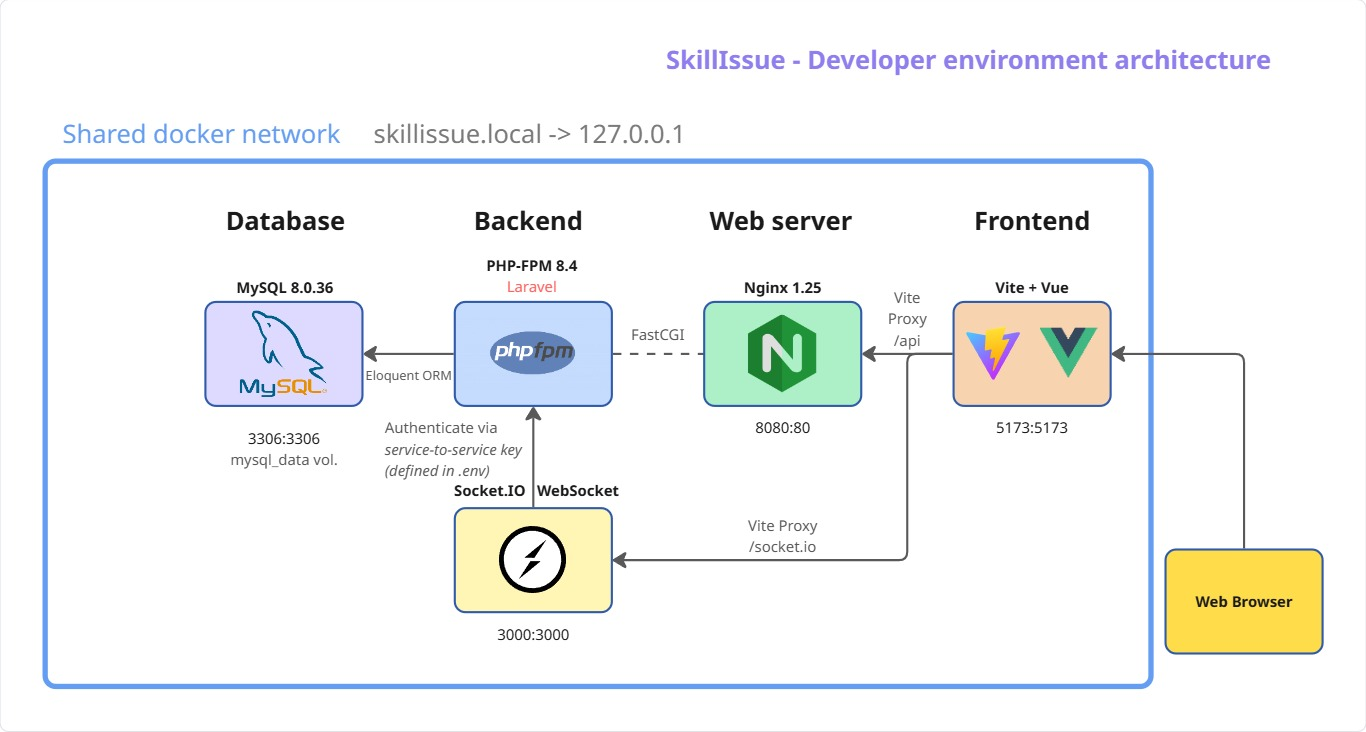
\includegraphics[width=\textwidth]{images/dev_diagram.png}
    \caption{A SkillIssue fejlesztői környezetének architektúrája}
    \label{fig:dev-architektura}
\end{figure}
\textbf{Megjegyzés:} Teszteléshez a SkillIssue weboldal is használható: https://skillissue.hu. Az alkalmazás jelszóval van védve:

\begin{center}
    \begin{tabular}{ll}
     \textbf{Felhasználónév} & skillissue \\
     \textbf{Jelszó} & neumanneger2026
    \end{tabular}
\end{center}

\section{Környezeti változók}
A környezeti változók három \texttt{.env} fájlban vannak tárolva:
\begin{description}
    \item[.env.dev] Fejlesztői környezet környezeti változói 
    \item[.env.prod] Éles környezet környezeti változói 
    \item[.env] A Dockerhez használatos környezeti változók, a jogosultság szinkronizálására a Docker konténer és a host számítógép között.
\end{description}
\newpage
\begin{center}
    \textit{Fontosabb Laravel környezeti változók}:\\
    \begin{tabular}{|c|l|}
        \hline
        \textbf{Környezeti változó neve} & \textbf{Leírás} \\
        \hline
        APP\_ENV & Lehetséges értéke: local, production. \\
        \hline
        APP\_KEY & Base64-el enkódolt kulcs, amit a Laravel alkalmazás titkosításra használ. \\
        \hline
        DB\_[*] & A Laravel által létrehozott adatbázis-kapcsolat paraméterei. \\
        \hline
        SESSION\_DRIVER & Pl.: cookie, database, file, stb. - Meghatározza, hol legyenek tárolva a session adatok. \\
        \hline
        SESSION\_LIFETIME & Session élettartama, percben. \\
        \hline
        SESSION\_ENCRYPT & Boolean, session adatok titkosított tárolása \\
        \hline
        SESSION\_PATH & A session cookie milyen URL-en legyen elérhető (/ = egész domain). \\
        \hline
        SESSION\_DOMAIN & Melyik domain-en legyen érvényes a session cookie. \\
        \hline
    \end{tabular}
\end{center}

\begin{center}
    \textit{Játékmenet és saját implementációkra vonatkozó környezeti változók:}\\
    \begin{tabular}{|c|l|}
        \hline
        \textbf{Környezeti változó neve} & \textbf{Leírás} \\
        \hline
        MAX\_ROUNDS & Hány körös legyen a mérkőzés (Solo és Ranked) \\
        \hline
        SOLO\_MAX\_GUESS\_TIME & Maximum válaszadási idő (másodperc, egyjátékos mód) \\
        \hline
        RANKED\_MAX\_GUESS\_TIME & Maximum válaszadási idő (másodperc, Ranked 1 vs. 1 mód) \\
        \hline
        SERVICE\_TOKEN & Service-to-service kommunikációhoz meghatározott közös token \\
        \hline
    \end{tabular}
\end{center}

A részletes dokumentáció megtalálható a \ref{ch:envvar} függelékben (Környezeti változók dokumentációja).

\section{Fejlesztői vs. Éles konfiguráció}
A konfigurációs különbségeket részletesen a \ref{sec:dockeconfig}. szakasz taglalja. 
\\
Összességében elmondható, hogy a \textbf{fejlesztői környezet} esetében az elsődleges szempont a könnyű elindítás, fejlesztés segítése, a hot-reload támogatása, parancssori eszközök (artisan) könnyű használatának biztosítása és a jogosultságok szinkronizálása. A fejlesztői környezetben az egységes munkavégzés érdekében \texttt{.prettierrc} Prettier konfigurációs fájl található, amely lehetővé teszi a kódbázis egységes formázását.
\\
Az \textbf{éles környezetben} a fő szempont az egyszerű szállítás, deployment, illetve a biztonság. 

\section{Makefile parancsok}
A hosszú parancsok kiküszöbölésének érdekében a Makefile segíti a fejlesztő munkáját. Hat részre van bontva: Dev, Migration, Build, Publish, Prod, Utils.
A Makefile összes utasítása és részletes leírása: \ref{ch:makefile} függelék (Makefile parancsok referencia)
\section{Tesztelési stratégia}

A SkillIssue projekt tesztelési stratégiájának kialakításakor a szűkös időkeret és a kétfős csapatméret jelentette a legnagyobb kihívást. Bár az alkalmazás egy MVP (Minimum Viable Product), a komplex, valós idejű WebSocket események, az összetett statisztikai számítások és a kritikus állapotkezelés megkövetelte a tesztelési szintek kombinálását. 

A tisztán manuális tesztelés helyett egy hibrid megközelítést alkalmaztunk. A backend üzleti logikáját (pl. statisztikák számítása, jogosultságkezelés) és a frontend legfontosabb komponenseit, illetve állapotkezelőit automatizált Unit és Feature tesztekkel védtük le. Ezzel párhuzamosan a valós idejű játékmenetet, a hálózati anomáliákat és a felhasználói élményt kiterjedt manuális teszteléssel validáltuk. Ez a stratégia biztosította, hogy az alapvető funkciók stabilak maradjanak a fejlesztés során, miközben az edge-case-ek is feltárásra kerültek.

\section{Manuális tesztelés}

A manuális tesztelési folyamat két jól elkülöníthető fázisban és módszertannal valósult meg a projekt során.

\begin{description}
    \item[Fejlesztői tesztelés (WhiteBox megközelítés)] Az első ágat a kódismereten alapuló tesztelés jelentette. Minden kódmódosítás, refaktorálás vagy új funkció implementálása után, a rendszerarchitektúra pontos ismeretének fényében vizsgáltuk az alkalmazást. A tesztelés során célzottan azokat a modulokat és API végpontokat terheltük, amelyekre az adott módosítások a legnagyobb eséllyel hatással lehettek. Ezzel a módszerrel a UI hibák és a hálózati deszinkronizációk nagy része már a fejlesztői környezetben kiküszöbölésre került.

    \item[Harmadik fél általi tesztelés (BlackBox megközelítés)] A rendszer komplexitásából és a valós idejű játékmenetből adódóan a fejlesztői tesztelés önmagában nem volt elegendő. Bevontunk harmadik feleket (diáktársakat, barátokat) is a tesztelési folyamatba, akiknek az volt a feladatuk, hogy a kódbázis ismerete nélkül, átlagos felhasználóként navigáljanak az oldalon. Megpróbáltak lejátszani egyjátékos és rangsorolt meccseket, valamint váratlan interakciókkal "elrontani" a rendszert. Számos olyan hibára (például a böngészőlap meccs közbeni frissítése vagy a hálózati megszakadások kezelése) derült fény, amelyek javítása elengedhetetlen volt egy stabil alkalmazás kiadásához.
\end{description}

\section{Automatizált tesztelés}

Az automatizált tesztek feladata a regressziós hibák elkerülése, a kritikus backend üzleti logika hibátlan működésének garantálása, és a frontend állapotkezelésének validálása volt. A teszteket két fő részre bontottuk: a backend tesztek a PHPUnit keretrendszerrel, míg a frontend tesztek a Vitest és a Vue Test Utils segítségével készültek.

\subsection{Backend tesztek (Laravel / PHPUnit)}

A backend automatizált tesztjei elsősorban a jogosultságkezelésre, a mérkőzések érvényesítésére (JWT tokenek), valamint a felhasználói statisztikák (Win rate, Elo) pontos kiszámítására fókuszálnak.

\begin{table}[h!]
    \centering
    \small
    \begin{tabularx}{\textwidth}{|l|X|X|}
        \hline
        \rowcolor[HTML]{EFEFEF} 
        \textbf{Tesztfájl / Osztály} & \textbf{Típus} & \textbf{Leírás és vizsgált funkciók} \\ \hline
        
        \multicolumn{3}{|l|}{\cellcolor[HTML]{F5F5F5}\textit{Autentikáció és Jogosultságok (Feature)}} \\ \hline
        \texttt{AuthTest} & Feature & Regisztráció, bejelentkezés, helytelen jelszó kezelése, email validáció, kijelentkezés és a védett útvonalak (Auth middleware) tesztelése. \\ \hline
        \texttt{AdminAccessTest} & Feature & Ellenőrzi, hogy csak az adminisztrátorok férhetnek hozzá a védett végpontokhoz (pl. tantárgyak létrehozása, felhasználók tiltása - Ban, meccsek törlése). \\ \hline
        
        \multicolumn{3}{|l|}{\cellcolor[HTML]{F5F5F5}\textit{Játékmenet és Működés (Feature)}} \\ \hline
        \texttt{VerifyAnswerTest} & Feature & Komplex teszt a válaszok beküldésére. Validálja a többszörös JWT tokeneket (Question, Practice Session, Ranked, Service tokenek) és az adatbázis frissülését. \\ \hline
        \texttt{UserReportTest} & Feature & Megbizonyosodik róla, hogy a felhasználók megfelelően tudnak mérkőzéseket és kérdéseket jelenteni érvényes azonosítókkal. \\ \hline
        \texttt{HealthTest} & Feature & A rendszer alapvető elérhetőségét (Health check) vizsgálja. \\ \hline

        \multicolumn{3}{|l|}{\cellcolor[HTML]{F5F5F5}\textit{Üzleti Logika (Unit)}} \\ \hline
        \texttt{UserCalculationTest} & Unit & A felhasználói statisztikák (Győzelmi arány, Win streak, Pontosság) és a rangok (Elo rendszer) számításának ellenőrzése. Vizsgálja a kitiltás (Ban) állapotának helyes lekérdezését is. \\ \hline
    \end{tabularx}
    \caption{Backend automatizált tesztek és azok funkciói}
\end{table}

\subsection{Frontend tesztek (Vue 3 / Vitest)}

A frontend tesztek célja a Pinia store-ok (állapotkezelés) és a Vue komponensek megfelelő renderelésének és interaktivitásának biztosítása.

\begin{table}[h!]
    \centering
    \small
    \begin{tabularx}{\textwidth}{|l|X|X|}
        \hline
        \rowcolor[HTML]{EFEFEF} 
        \textbf{Tesztfájl / Osztály} & \textbf{Érintett Modul} & \textbf{Leírás és vizsgált funkciók} \\ \hline
        
        \multicolumn{3}{|l|}{\cellcolor[HTML]{F5F5F5}\textit{Állapotkezelés és Útválasztás}} \\ \hline
        \texttt{UserStore.spec.js} & Pinia Store & Munkamenet ellenőrzése (\texttt{verifySession}), sikeres bejelentkezés állapota. Kiemelten kezeli a 401-es hibát (automatikus kijelentkezés) és a WebSocket kapcsolat megfelelő felépítését, illetve bontását (logout esetén). \\ \hline
        \texttt{router.spec.js} & Vue Router & Router Guard-ok tesztelése. Ellenőrzi, hogy az autentikálatlan felhasználók a login oldalra, a jogosulatlanok pedig az admin oldalról a főoldalra lesznek-e átirányítva. \\ \hline
        
        \multicolumn{3}{|l|}{\cellcolor[HTML]{F5F5F5}\textit{Komponensek és Interakciók}} \\ \hline
        \texttt{SoloWidget.spec.js} & UI Komponens & Egyjátékos modul. Teszteli a kérdések és adatok helyes renderelését, a válaszadás gomb működését (\texttt{emit}), a hiányzó válasz esetén felugró hibaüzeneteket, és a jelentés megnyitását. \\ \hline
        \texttt{RankedWidget.spec.js} & UI Komponens & Rangsorolt widget működése, a GameStore-ral való megfelelő integráció, valamint a válaszok helyes API beküldésének szimulációja. \\ \hline
        \texttt{QuestionReport.spec.js} & UI Komponens & Kérdésjelentő űrlap tesztje: megjelenítés, üres mezők validációja (hibaüzenet-megjelenítés), valamint API hívások paramétereinek és a beküldés sikerességének (isSubmitted) ellenőrzése. \\ \hline
    \end{tabularx}
    \caption{Frontend automatizált tesztek és azok funkciói}
\end{table}
\chapter{Összefoglalás}

\section{Megvalósított funkciók}
Végeredményben a rendszer egy komplex kvízalkalmazást valósít meg, mely egyesíti a többjátékos kompetitív élményt oktatási funkciókkal. A rendszer központi elemei a valós idejű rangsorolt játékmenet, a fejlődés nyomonkövetését elősegítő rendszerek valamint az adminisztrációs rendszer.

A rendszer a következő funkciókat valósítja meg:
\begin{itemize}
    \item Reszponzív viselkedésforma
    \item Regisztráció, Autentikáció
    \item Játékosprofilok
    \item ELO rangrendszer
    \item XP rendszer
    \item Daily streak (napi sorozat) számítás
    \item Winstreak (nyerési sorozat) számítás
    \item Egyjátékos gyakorló meccsek
    \item Többjátékos meccskeresési funkció (SBMM)
    \item 1 vs. 1 rangsorolt mérkőzések
    \item Játékos -és kérdés bejelentési funkciók
    \item Jogosultságrendszer
    \item Adminisztrációs rendszer
\end{itemize}

\section{Nehézségek és tanulságok}
A rendszer komplexitása miatt több helyen is szükség volt kreativitásra a problémák megoldása érdekében:

\begin{itemize}
    \item \textbf{Egyszerű csalásra használható scriptek kiküszöbölése:} A lehető legminimálisabb információkat szabad közölni a klienssel, annak érdekében, hogy az automatizált csalásokat - amelyek a hálózati kéréseket figyelik - kiküszöbölje a rendszer.
    \item \textbf{Valós idejű játékmenet:} Edge case-ek kiküszöbölése: játékos nem fogadja el a meccset, kilép, visszacsatlakozik, több lapon használja az alkalmazást. 
    \item \textbf{Meccskeresés:} Fair, jól balance-olt rendszer kialakítása, minimális erőforrásigénnyel.
    \item \textbf{Tesztelés:} A sok funkció manuális tesztelése nehézkes volt, ami rávilágított az automatizált tesztek fontosságára.
\end{itemize}

\newpage

\section{Továbbfejlesztési lehetőségek}
A rendszer jelenlegi állapota egy MVP-t (Minimum viable product) valósít meg. A rendszer számos továbbfejlesztési lehetőséggel rendelkezik, amelynél a fő szempontok a következők: csalás kiküszöbölése, SBMM továbbfejlesztése, játékmódok bővítése.

Néhány példa továbbfejlesztési lehetőségekre:
\begin{itemize}
    \item \textbf{Csalás kiküszöbölése:} Rangsorolt meccs folyamán több adat rögzítése, annak érdekében, hogy könnyebben eldönthető lehessen, hogy csalt-e a játékos. Például: Focus loss detection (játékos elhagyja-e az oldalt meccs közben - "tab-out"), pontosabb guess time számítás.
    \item \textbf{Új játékmódok:} Olyan játékmódok bevezetése, amelyek elősegítik a tanulást: CO-OP játékmód, ahol több játékos együttes munkával megismer egy adott érettségi témát; csoportos kompetitív játékmódok.
    \item \textbf{Kérdések bővítése:} Olyan közösségi felület, ahol a játékosok kérdéseket javasolhatnak.
    \item \textbf{Mobilapplikáció:} Android, iOS alkalmazás fejlesztése a jobb felhasználói élmény érdekében, például Flutter segítségével.
    \item \textbf{Badge és Achievement rendszer:} Bizonyos mérföldkövek után a játékos Badge-eket kap, amelyek megjelennek a profiljukon, ezzel növelve a motivációt. (A Badge rendszer adatbázis struktúrája megtalálható az MVP-ben, de a implementálásra nem kerül)
    \item \textbf{Távoli jövő - teljes érettségi felkészítő platform:} Monetizált érettségi felkészítő platform, ahol a jelenleg ismertetett funkciókon kívül megtalálható hivatalos tanári segítség és több erőforrás a tanuló felkészülésének elősegítése érdekében.
\end{itemize}

\appendix
\include{appendix-api-ref}
\chapter{Környezeti változók dokumentációja}
\label{ch:envvar}

A rendszer konfigurációja környezeti változókon keresztül történik, amelyeket a \texttt{.env} fájlok tartalmaznak. Külön fájl szolgál a Docker környezethez (\texttt{.env}), a fejlesztéshez (\texttt{.env.dev}) és az éles üzemhez (\texttt{.env.prod}).

\begin{table}[h!]
    \centering
    \small
    \renewcommand{\arraystretch}{1.3}
    \begin{tabularx}{\textwidth}{|l|X|X|}
        \hline
        \rowcolor[HTML]{EFEFEF} 
        \textbf{Változó} & \textbf{Alapértelmezett / Példa} & \textbf{Leírás} \\ \hline
        
        \multicolumn{3}{|l|}{\cellcolor[HTML]{F5F5F5}\textit{Docker (Alapkonfiguráció)}} \\ \hline
        \texttt{UID / GID} & \texttt{1000} & A gazdagép felhasználói és csoport azonosítója a fájljogosultságokhoz. \\ \hline
        
        \multicolumn{3}{|l|}{\cellcolor[HTML]{F5F5F5}\textit{Alkalmazás (Laravel)}} \\ \hline
        \texttt{APP\_NAME} & \texttt{SkillIssue} & Az alkalmazás megnevezése. \\ \hline
        \texttt{APP\_ENV} & \texttt{local / production} & A futtatási környezet típusa. \\ \hline
        \texttt{APP\_KEY} & \texttt{base64:...} & Az alkalmazás titkosító kulcsa (\texttt{make dev-key}). \\ \hline
        \texttt{APP\_URL} & \texttt{https://skillissue.hu} & Az alkalmazás elérési útvonala. \\ \hline
        \texttt{APP\_DEBUG} & \texttt{true / false} & Hibakeresési mód ki- és bekapcsolása. \\ \hline
        
        \multicolumn{3}{|l|}{\cellcolor[HTML]{F5F5F5}\textit{Adatbázis (MySQL)}} \\ \hline
        \texttt{DB\_CONNECTION} & \texttt{mysql} & Az adatbázis-kezelő típusa. \\ \hline
        \texttt{DB\_HOST} & \texttt{mysql} & Az adatbázis-szolgáltatás gépneve (Docker-en belül). \\ \hline
        \texttt{DB\_DATABASE} & \texttt{skillissue} & A használt adatbázis neve. \\ \hline
        \texttt{DB\_USERNAME} & \texttt{root / appuser} & Az adatbázis eléréséhez használt felhasználónév. \\ \hline
        \texttt{DB\_PASSWORD} & \texttt{********} & Az adatbázis jelszava. \\ \hline
        
        \multicolumn{3}{|l|}{\cellcolor[HTML]{F5F5F5}\textit{Játékmechanika}} \\ \hline
        \texttt{MAX\_ROUNDS} & \texttt{5} & Egy mérkőzés maximális köreinek száma. \\ \hline
        \texttt{SOLO\_MAX\_GUESS\_TIME} & \texttt{30} & Válaszadási idő másodpercben (gyakorló mód). \\ \hline
        \texttt{RANKED\_MAX\_GUESS\_TIME} & \texttt{30} & Válaszadási idő másodpercben (rangsorolt mód). \\ \hline
        \texttt{VITE\_*} & \texttt{...} & A frontend számára is elérhetővé tett változók (prefixelt). \\ \hline
        
        \multicolumn{3}{|l|}{\cellcolor[HTML]{F5F5F5}\textit{Biztonság és Kommunikáció}} \\ \hline
        \texttt{SERVICE\_TOKEN} & \texttt{abcdefg123456} & A belső szolgáltatások (API és WebSocket) közötti hitelesítéshez. \\ \hline
        \texttt{SANCTUM\_STATEFUL\_DOMAINS} & \texttt{skillissue.hu, ...} & Engedélyezett domainek a sütialapú hitelesítéshez. \\ \hline
    \end{tabularx}
    \caption{A projektben használt legfontosabb környezeti változók}
\end{table}

\noindent \textbf{Fontos:} Éles környezetben (\texttt{.env.prod}) a \texttt{SESSION\_ENCRYPT} értéke kötelezően \texttt{true}, a \texttt{LOG\_LEVEL} pedig \texttt{warning} szintre van állítva a biztonság és a teljesítmény érdekében.
\chapter{Makefile parancsok referencia}
\label{ch:makefile}

A projekt gyökérkönyvtárában található \texttt{Makefile} segítségével egyszerűsíthetők a gyakran ismételt Docker, Laravel és karbantartási feladatok. Az alábbi táblázat összefoglalja a rendelkezésre álló parancsokat és azok funkcióit.

\begin{table}[h!]
    \centering
    \small
    \begin{tabularx}{\textwidth}{|l|X|X|}
        \hline
        \rowcolor[HTML]{EFEFEF} 
        \textbf{Parancs} & \textbf{Futtatott művelet} & \textbf{Leírás} \\ \hline
        
        \multicolumn{3}{|l|}{\cellcolor[HTML]{F5F5F5}\textit{Fejlesztői környezet (DEV)}} \\ \hline
        \texttt{make dev-key} & \texttt{docker compose run artisan key:generate} & Új Laravel \texttt{APP\_KEY} generálása a fejlesztői környezethez. \\ \hline
        \texttt{make dev-up} & \texttt{docker compose up -{}-build} & Konténerek indítása az előtérben, kényszerített újraépítéssel. \\ \hline
        \texttt{make dev-up-d} & \texttt{docker compose up -d} & Konténerek indítása a háttérben (detached mód). \\ \hline
        \texttt{make dev-down} & \texttt{docker compose down} & Fejlesztői konténerek leállítása. \\ \hline
        \texttt{make dev-down-v} & \texttt{docker compose down -v} & Leállítás és az adatbázis volume-ok teljes törlése. \\ \hline
        
        \multicolumn{3}{|l|}{\cellcolor[HTML]{F5F5F5}\textit{Adatbázis műveletek (MIGRATE)}} \\ \hline
        \texttt{make migrate} & \texttt{./artisan migrate} & Új adatbázis migrációk futtatása. \\ \hline
        \texttt{make migrate-seed} & \texttt{./artisan migrate -{}-seed} & Migrálás és alapértelmezett adatok feltöltése. \\ \hline
        \texttt{make migrate-fresh} & \texttt{./artisan migrate:fresh} & Összes tábla törlése és migrációk újrafuttatása. \\ \hline
        \texttt{make migrate-fresh-seed} & \texttt{./artisan migrate:fresh -{}-seed} & Teljes alaphelyzetbe állítás tesztadatok betöltésével. \\ \hline
        
        \multicolumn{3}{|l|}{\cellcolor[HTML]{F5F5F5}\textit{Build \& Publish}} \\ \hline
        \texttt{make build} & \texttt{docker build -t ...} & Éles Docker image-ek összeállítása (opcionális verziózással). \\ \hline
        \texttt{make push} & \texttt{docker push ...} & Elkészült image-ek feltöltése a Docker Hub tárhelyre. \\ \hline
        \texttt{make release} & \texttt{make build push} & Verziózott kiadás gyártása és publikálása egy lépésben. \\ \hline
        
        \multicolumn{3}{|l|}{\cellcolor[HTML]{F5F5F5}\textit{Éles környezet (PROD)}} \\ \hline
        \texttt{make prod-up} & \texttt{docker compose up} & Éles környezet indítása az előtérben. \\ \hline
        \texttt{make prod-up-d} & \texttt{docker compose up -d} & Éles környezet indítása a háttérben. \\ \hline
        \texttt{make prod-pull} & \texttt{docker compose pull} & Legfrissebb image-ek letöltése a Docker Hub-ról. \\ \hline
        \texttt{make prod-db-seed} & \texttt{docker compose run artisan db:seed} & Éles adatbázis inicializálása (csak egyszeri futtatásra). \\ \hline
        
        \multicolumn{3}{|l|}{\cellcolor[HTML]{F5F5F5}\textit{Segédprogramok (UTILS)}} \\ \hline
        \texttt{make logs} & \texttt{docker compose logs -f} & Éles naplófájlok (\textit{logs}) folyamatos követése. \\ \hline
        \texttt{make ps} & \texttt{docker compose ps} & Futó konténerek és állapotuk listázása. \\ \hline
        \texttt{make prettier} & \texttt{npx prettier -{}-write ...} & Forráskód automatikus formázása (Frontend és Websocket). \\ \hline
    \end{tabularx}
    \caption{A projektben használt automatizációs parancsok listája}
\end{table}

\noindent \textbf{Megjegyzés:} A táblázatban szereplő \texttt{migrate} parancsok közvetlenül a gazdagépen futtatott \texttt{./artisan} scriptet használják, amely a megfelelő Docker konténerben hajtja végre a műveletet.

\end{document}
